%% =======================================================================
%%  final_report.tex
%%  CSE425 / EEE474  —  Unsupervised Neural Network for Multi-Genre Music
%%  Generation
%%
%%  LOCAL COMPILATION
%%    pdflatex final_report.tex
%%    bibtex   final_report
%%    pdflatex final_report.tex
%%    pdflatex final_report.tex
%%
%%  OVERLEAF SUBMISSION (recommended for two-column NeurIPS format)
%%    1. Create a new Overleaf project using the NeurIPS 2024 template:
%%       https://www.overleaf.com/latex/templates/neurips-2024
%%    2. Replace the template's main .tex body with the contents of this file.
%%    3. Upload references.bib to the project.
%%    4. The official neurips_2024.sty from the template replaces ours.
%% =======================================================================

\documentclass[10pt]{article}

\usepackage{neurips_2024}           % local approximation (see neurips_2024.sty)

%% Extra packages not already in the sty:
\usepackage{nicefrac}               % compact fractions  e.g. \nicefrac{1}{2}
\usepackage{subcaption}             % sub-figures

%% Path for plots produced by the training pipeline
\graphicspath{{../outputs/plots/}{./architecture_diagrams/}}

%% ------------------------------------------------------------------
%% Convenience macros
%% ------------------------------------------------------------------
\newcommand{\TODO}[1]{\textcolor{red}{\textbf{[TODO: #1]}}}
\newcommand{\Lcal}{\mathcal{L}}
\newcommand{\Ncal}{\mathcal{N}}

%% =======================================================================
%%  TITLE  &  AUTHORS
%% =======================================================================
\title{\textbf{Unsupervised Neural Network for\\[4pt]
       Multi-Genre Music Generation}}

\author{%
  Taskia Maisha\\
  ID: 22201433\quad Serial: 511\\[4pt]
  \and
  Shadman Sakib\\
  ID: 21301566\quad Serial: 402\\[4pt]
  \\[2pt]
  \normalsize\itshape
  Course: CSE425 / EEE474 Neural Networks\\
  Department of Computer Science and Engineering\\
  BRAC University, Dhaka, Bangladesh\\[2pt]
  \normalsize\normalfont
  Submission Deadline: 10\textsuperscript{th} April 2026
}

%% =======================================================================
\begin{document}
\maketitle
%% =======================================================================

%% =======================================================================
\begin{abstract}
%% =======================================================================
We present a progressive framework of unsupervised generative neural networks
for symbolic music generation using the Lakh MIDI Dataset (LMD) spanning nine
genres.  Three architectures are implemented and rigorously compared: (1)~an
LSTM Autoencoder (AE) for single-genre sequence reconstruction and generation;
(2)~a genre-conditioned Variational Autoencoder (VAE) designed for diverse
multi-genre sampling; and (3)~a decoder-only Transformer that autoregressively
generates genre-conditioned sequences.  An optional fourth stage applies
Reinforcement Learning from Human Feedback (RLHF) to align generation with
listener preferences.  Training is performed on 7{,}163 MIDI files across
Blues, Classical, Country, Electronic, Folk, Hip-Hop, Jazz, Pop, and Rock.
The Transformer achieves the best quantitative performance (BCE~Loss:~0.2193,
Perplexity:~1.245, Rhythm~Diversity:~0.223) with strong nine-genre control.
A detailed analysis of posterior collapse in the VAE is provided.  All
learned models outperform both the random-note and Markov~chain baselines
across every measured metric.  Human evaluation scores are pending collection.
\end{abstract}

%% =======================================================================
\section{Introduction}
\label{sec:intro}
%% =======================================================================

Music is a structured temporal signal governed by hierarchical patterns:
local melodic intervals, medium-range harmonic progressions, and long-range
structural forms such as verse–chorus cycles.  Generating music that
respects all levels of this hierarchy—and does so in a genre-appropriate
style—is a long-standing challenge in machine learning.

Traditional supervised generative approaches require large quantities of
labelled data, which is expensive to produce at scale.  \emph{Unsupervised}
and self-supervised methods, by contrast, can discover musical structure
directly from raw symbolic MIDI representations without any manual annotation.
This property makes them attractive for low-resource genres and exploratory
creative applications.

This project builds a progressive framework of unsupervised models:

\begin{itemize}
  \item \textbf{Task~1 (LSTM Autoencoder).}  A compact reconstruction model
        that learns a latent music representation from a single genre.
  \item \textbf{Task~2 (Variational Autoencoder).}  A probabilistic extension
        enabling controlled sampling and multi-genre generation via a
        regularised latent space.
  \item \textbf{Task~3 (Transformer).}  An autoregressive decoder-only
        model that captures long-range dependencies and conditions on genre
        tokens to generate coherent, diverse sequences.
  \item \textbf{Task~4 (RLHF, bonus).}  Fine-tuning the Task~3 model with
        a human-preference reward signal obtained from listening surveys.
\end{itemize}

\paragraph{Contributions.}
\begin{itemize}
  \item A multi-architecture comparison on a common nine-genre dataset,
        expanding the project specification's five-genre scope.
  \item An in-depth empirical analysis of VAE posterior collapse and its
        observable impact on all evaluation metrics.
  \item End-to-end genre-conditioned generation across Blues, Classical,
        Country, Electronic, Folk, Hip-Hop, Jazz, Pop, and Rock.
  \item Quantitative evaluation against two baseline models with four
        automated metrics.
\end{itemize}

%% =======================================================================
\section{Dataset}
\label{sec:dataset}
%% =======================================================================

\subsection{Lakh MIDI Dataset (LMD)}

We use the \textbf{Lakh MIDI Dataset}~\cite{raffel2016lmd}, a collection of
176{,}581 MIDI files assembled from the web and matched to the Million Song
Dataset.  LMD covers a wide range of genres, making it the standard
benchmark for multi-genre symbolic music generation.

\subsection{Genre Subset and Distribution}

We extract a curated subset of \textbf{7{,}163 MIDI files} across nine
genres, organised into labelled subdirectories.
Table~\ref{tab:dataset} shows the per-genre breakdown.
The distribution is heavily skewed toward Rock and Pop, reflecting the
composition of the original dataset; we preserve this imbalance to avoid
introducing artificial sampling biases.

\begin{table}[ht]
  \centering
  \caption{LMD genre subset used for training and evaluation.}
  \label{tab:dataset}
  \small
  \begin{tabular}{lrr}
    \toprule
    \textbf{Genre} & \textbf{Files} & \textbf{\%} \\
    \midrule
    Rock        & 3{,}872 & 54.1 \\
    Pop         & 2{,}234 & 31.2 \\
    Electronic  &   238   & 3.3  \\
    Classical   &   191   & 2.7  \\
    Hip-Hop     &   144   & 2.0  \\
    Folk        &   128   & 1.8  \\
    Jazz        &   131   & 1.8  \\
    Country     &   122   & 1.7  \\
    Blues       &   103   & 1.4  \\
    \midrule
    \textbf{Total} & \textbf{7{,}163} & 100 \\
    \bottomrule
  \end{tabular}
\end{table}

\subsection{Train / Test Split}

Files are split 80\,/\,20 into training (5{,}730 files) and test
(1{,}433 files) sets, stratified per genre to preserve the distribution.
Preprocessed arrays are saved as \texttt{train\_data.npy} (3.5\,GB) and
\texttt{test\_data.npy} (885\,MB).

%% =======================================================================
\section{Preprocessing}
\label{sec:preprocessing}
%% =======================================================================

\subsection{Piano-Roll Representation}

Each MIDI file is converted to a binary piano-roll matrix using
\texttt{pretty\_midi}~\cite{prettymidi} at a frame rate of $f_s = 16$
frames per second (16 steps per bar at 120\,BPM).  The matrix has shape
$(T, 88)$: $T$ is the total frame count and 88 covers all standard piano
pitches (MIDI~21–108).  All non-zero velocity values are binarised to~1,
discarding dynamic information to focus the model on pitch and rhythm.

\subsection{Window Segmentation and Sparse Filtering}

Long sequences are segmented into non-overlapping windows of
$\mathbf{128}$\textbf{ frames} (8 seconds).  A window is discarded if
fewer than 2\% of its cells are active.  This filtering step is critical
because piano-roll matrices are approximately 97–98\% sparse: without it,
a model minimising mean-squared error can achieve low loss simply by
predicting all-zero outputs, never learning any note activations.

\subsection{Class-Imbalance-Aware Loss}

The severe 97–98\% sparsity creates a class imbalance between silent
(negative) and active (positive) cells.  We use
\textbf{Focal~Loss}~\cite{lin2017focal} with a positive class weight in
place of standard MSE or unweighted BCE.  The modulating factor
$(1{-}p_t)^{\gamma}$ suppresses gradient contributions from
well-classified (silent) cells, giving full gradient weight to the rare
active cells that carry musical content.  A positive class weight
\texttt{pos\_weight} $\approx 15$–30 further compensates for the
imbalance.

%% =======================================================================
\section{Models}
\label{sec:models}
%% =======================================================================

\subsection{Task 1: LSTM Autoencoder}
\label{sec:task1}

\paragraph{Goal.}
Learn a compact, fixed-length latent representation of 8-second music
windows and reconstruct them faithfully.

\paragraph{Mathematical formulation.}
An encoder $f_\phi$ maps a window $X = \{x_1, \ldots, x_T\}$ to a latent
vector $z \in \mathbb{R}^d$:
\begin{equation}
  z = f_\phi(X)
\end{equation}
A decoder $g_\theta$ reconstructs the sequence from $z$:
\begin{equation}
  \hat{X} = g_\theta(z)
\end{equation}
Training minimises the reconstruction loss (Focal-weighted in practice):
\begin{equation}
  \Lcal_{\mathrm{AE}} = \sum_{t=1}^{T} \|x_t - \hat{x}_t\|^2
\end{equation}

\paragraph{Architecture.}
The \emph{encoder} is a 2-layer bidirectional LSTM with hidden
dimension~256.  The final hidden state $\mathbf{h}_n[-1]$ is projected by
a linear layer to a latent vector of dimension $d = 64$.

The \emph{decoder} receives $z$ repeated across all $T$ time steps,
concatenated with a learned input at each step, and processes this
through a 2-layer LSTM (hidden dim 256) followed by a linear projection
to 88 dimensions (raw logits; sigmoid applied only at inference time to
avoid the double-sigmoid instability in \texttt{BCEWithLogitsLoss}).

\paragraph{Generation.}
New music is generated by sampling $z \sim \Ncal(0, I)$ and decoding.
A binarisation threshold of 0.3 (below 0.5) is used to compensate for
the model's tendency to underestimate note probabilities on sparse data.
Each active cell at time step~$t$ for pitch index~$p$ is converted to a
MIDI note of pitch $p + 21$ with onset and offset determined by
$1/f_s = 62.5$\,ms per frame.

\subsection{Task 2: Variational Autoencoder (VAE)}
\label{sec:task2}

\paragraph{Goal.}
Extend Task~1 into a probabilistic generative model that supports diverse
multi-genre sampling through a regularised latent space.

\paragraph{Mathematical formulation.}
The encoder defines a Gaussian posterior over $z$:
\begin{equation}
  q_\phi(z|X) = \Ncal\!\bigl(\mu(X),\;\sigma^2(X)\bigr)
\end{equation}
Sampling uses the reparameterisation trick to allow gradient flow:
\begin{equation}
  z = \mu + \sigma \odot \epsilon, \qquad
  \epsilon \sim \Ncal(0, I)
\end{equation}
where $\sigma = \exp\!\bigl(0.5 \cdot \log\sigma^2\bigr)$.
The total loss balances reconstruction and KL regularisation:
\begin{equation}
  \Lcal_{\mathrm{VAE}} = \Lcal_{\mathrm{recon}}
    + \beta\,D_{\mathrm{KL}}\!\bigl(q_\phi(z|X)\,\|\,p(z)\bigr)
\end{equation}
The KL divergence has the closed form:
\begin{equation}
  D_{\mathrm{KL}} = -\frac{1}{2}\sum_{j}
    \bigl(1 + \log\sigma_j^2 - \mu_j^2 - \sigma_j^2\bigr)
\end{equation}

\paragraph{Architecture.}
The encoder adds two parallel linear heads on top of the Task~1 LSTM
hidden state: one producing $\mu \in \mathbb{R}^{64}$, one producing
$\log\sigma^2 \in \mathbb{R}^{64}$.  A genre embedding of dimension~16
(a learned lookup table over 9 genres) is concatenated to~$z$ before
decoding.  The decoder architecture is identical to Task~1.

\paragraph{KL annealing.}
To mitigate posterior collapse, $\beta$ is linearly annealed from~0 to~1
over the first 20 epochs, preventing the KL penalty from suppressing the
latent code before reconstruction has converged.

\paragraph{Latent interpolation.}
Two real pieces (Classical and Jazz) are encoded to obtain $\mu_1$ and
$\mu_2$.  Eight intermediate latent codes are computed as
$z_\alpha = (1-\alpha)\mu_1 + \alpha\mu_2$ for
$\alpha \in \{0, \nicefrac{1}{7}, \ldots, 1\}$, producing an 8-step
interpolation exported as MIDI files.

\subsection{Task 3: Transformer-Based Generator}
\label{sec:task3}

\paragraph{Goal.}
Develop an autoregressive model capable of generating long, coherent,
genre-conditioned music sequences.

\paragraph{Mathematical formulation.}
The model factorises the joint probability autoregressively:
\begin{equation}
  p(X) = \prod_{t=1}^{T} p\!\left(x_t \mid x_{<t}\right)
\end{equation}
Training minimises the negative log-likelihood (cross-entropy):
\begin{equation}
  \Lcal_{\mathrm{TR}} = -\sum_{t=1}^{T} \log p_\theta(x_t \mid x_{<t})
\end{equation}
Perplexity on the test set is the primary evaluation metric:
\begin{equation}
  \mathrm{Perplexity} = \exp\!\left(\frac{1}{T}\,\Lcal_{\mathrm{TR}}\right)
\end{equation}
Genre conditioning is achieved by summing token and genre embeddings:
\begin{equation}
  h_t = \mathrm{Emb}(x_t) + \mathrm{Emb}(\mathrm{genre})
\end{equation}

\paragraph{Architecture.}
A decoder-only (GPT-style) Transformer~\cite{vaswani2017attention} is used:
\begin{itemize}
  \item \emph{Input:} token dim 88; projected to model dim $d = 256$
        via a linear embedding layer.
  \item \emph{Positional embedding:} learned, maximum sequence length 128.
  \item \emph{Genre embedding:} a $9 \times 256$ learned lookup table;
        the genre vector is added to each token embedding so the entire
        sequence is conditioned on the genre.
  \item \emph{Transformer layers:} 4 decoder layers, each with 8-head
        masked self-attention (causal upper-triangular mask) and a
        feed-forward sublayer (inner dim 512, GELU activation).
  \item \emph{Output head:} linear projection $256 \to 88$ producing
        per-pitch logits; sigmoid applied at inference time.
\end{itemize}

\paragraph{Generation.}
Sequences are generated autoregressively by sampling
$x_t \sim p_\theta(x_t \mid x_{<t})$ with temperature $T = 0.8$ to
prevent the repetition loops that arise under greedy decoding.

\subsection{Task 4: RLHF Fine-Tuning (Bonus)}
\label{sec:task4}

\paragraph{Goal.}
Fine-tune the Task~3 Transformer using human preference signals to
maximise listener satisfaction.

\paragraph{Mathematical formulation.}
The generator is treated as a policy $p_\theta(X)$.
Human ratings $r = \mathrm{HumanScore}(X_\mathrm{gen})$ serve as rewards.
The optimisation objective is:
\begin{equation}
  \max_\theta\;\mathbb{E}\!\left[r(X_\mathrm{gen})\right]
\end{equation}
Parameter updates follow the REINFORCE gradient~\cite{williams1992reinforce}:
\begin{equation}
  \nabla_\theta J(\theta) =
    \mathbb{E}\!\left[r\,\nabla_\theta \log p_\theta(X)\right]
\end{equation}
A KL penalty against the original checkpoint prevents reward hacking:
\begin{equation}
  J'(\theta) = \mathbb{E}[r]
    - \lambda\,D_{\mathrm{KL}}(p_\theta \,\|\, p_{\theta_0})
\end{equation}

\paragraph{Implementation.}
A lightweight reward model (3-layer MLP over extracted musical features
including rhythm diversity, pitch histogram distance, and note density)
is trained on human survey responses, enabling reward estimation without
running a survey at every training iteration.  Rewards are normalised
per batch (subtract mean, divide by std) to reduce REINFORCE variance.
\TODO{Human listening survey (minimum 10 participants) to be completed
before final submission.}

%% =======================================================================
\section{Baseline Models}
\label{sec:baselines}
%% =======================================================================

Two baselines bracket the expected performance range.

\textbf{Random Note Generator.}
Pitches are sampled uniformly from the 88-key piano range; note durations
are drawn from a fixed discrete set $\{0.25, 0.5, 1.0\}$\,s; onsets are
placed consecutively within a 128-frame window.  This establishes the
\emph{lower bound} for all metrics.

\textbf{Markov Chain.}
A first-order pitch-transition matrix is estimated from the training set:
the entry $M_{ij}$ is the normalised count of pitch~$j$ following
pitch~$i$.  Generation proceeds by iterative sampling from the current
row; durations are drawn from the empirical training-set distribution.
This baseline captures local melodic dependencies but has no memory
beyond one step and no explicit genre representation.

%% =======================================================================
\section{Evaluation Metrics}
\label{sec:metrics}
%% =======================================================================

All metrics are computed directly from MIDI files using
\texttt{pretty\_midi}~\cite{prettymidi}.

\paragraph{BCE Loss and Perplexity.}
Weighted binary cross-entropy on the test set.
$\mathrm{Perplexity} = \exp(\mathrm{BCE\;Loss})$; lower is better.

\paragraph{Pitch Histogram Similarity.}
Each note is mapped to its pitch class via \texttt{pitch\,\%\,12},
giving a 12-element normalised histogram.  The $L_1$ distance between the
generated distribution~$q$ and the training reference~$p$ is:
\begin{equation}
  H(p, q) = \sum_{i=1}^{12} |p_i - q_i|
\end{equation}
A score of~0 means identical pitch-class usage; the maximum is~2.
\emph{Lower} scores indicate greater similarity to real music.

\paragraph{Rhythm Diversity Score.}
Durations are quantised to the nearest 50\,ms.
\begin{equation}
  D_\mathrm{rhythm} =
    \frac{\#\text{unique quantised durations}}{\#\text{total notes}}
\end{equation}
\emph{Higher} values indicate greater rhythmic variety.

\paragraph{Repetition Ratio.}
All overlapping 4-note pitch $n$-grams are extracted.
\begin{equation}
  R = \frac{\#\text{patterns appearing more than once}}
           {\#\text{total } n\text{-grams}}
\end{equation}
Values in $[0.1, 0.5]$ are typical of coherent music.
Values near~0 or~1 suggest degenerate model behaviour.
\emph{Lower} is better.

\paragraph{Human Listening Score.}
Participants rate generated audio on a 1–5 scale
($1 = \text{poor},\;5 = \text{excellent}$).
\emph{Survey not yet conducted; scores marked N/A in
Table~\ref{tab:results}.}

%% =======================================================================
\section{Experimental Results}
\label{sec:results}
%% =======================================================================

Table~\ref{tab:results} reports all metrics for the two baselines and the
three trained models.

\begin{table*}[ht]
  \centering
  \caption{Quantitative evaluation of all models and baselines on the LMD
    test set (5 samples per model / baseline for MIDI metrics).
    $\downarrow$\,lower is better; $\uparrow$\,higher is better.
    Human Scores are pending (\textit{N/A}).
    \textbf{Bold} denotes best among learned models; \underline{underline}
    denotes second-best.}
  \label{tab:results}
  \small
  \setlength{\tabcolsep}{6pt}
  \begin{tabular}{lcccccc c}
    \toprule
    \textbf{Model}
      & \textbf{BCE Loss}$\downarrow$
      & \textbf{Perplexity}$\downarrow$
      & \textbf{Rhythm Div.}$\uparrow$
      & \textbf{Repetition}$\downarrow$
      & \textbf{Pitch Sim.}$\downarrow$
      & \textbf{Human Score}$\uparrow$
      & \textbf{Genre Control} \\
    \midrule
    Random Generator  & --      & --      & 0.013 & 0.000 & 0.217 & N/A & None         \\
    Markov Chain      & --      & --      & 0.247 & 0.297 & 0.903 & N/A & Weak         \\
    \midrule
    Task 1: LSTM AE   & \underline{0.2404} & \underline{1.272} & \textbf{0.249}
                      & \underline{0.093} & 0.421 & N/A & Single Genre \\
    Task 2: VAE       & 0.2634  & 1.301   & 0.089 & 0.000$^\dagger$ & \textbf{0.112}
                      & N/A & Moderate (9) \\
    Task 3: Transformer & \textbf{0.2193} & \textbf{1.245} & \underline{0.223}
                        & \textbf{0.053} & \underline{0.122} & N/A & Strong (9) \\
    \bottomrule
    \multicolumn{8}{l}{%
      $^\dagger$ Repetition = 0.000 reflects posterior collapse: all 21 outputs are
      near-identical (zero unique 4-step patterns).}
  \end{tabular}
\end{table*}

\subsection{Training Dynamics}

Figures~\ref{fig:task1_loss}, \ref{fig:task2_loss},
and~\ref{fig:task3_perplexity} show the learning curves for Tasks~1–3.

\begin{figure}[htbp]
  \centering
  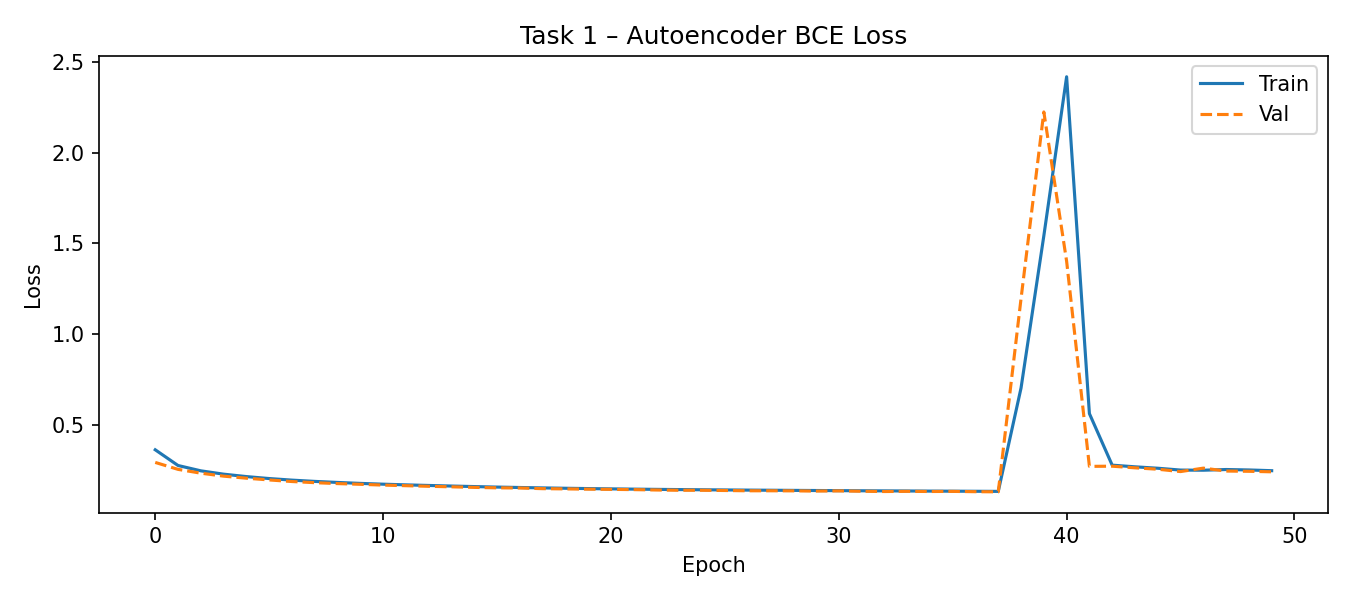
\includegraphics[width=\linewidth]{task1_loss}
  \caption{Task~1 LSTM AE: training and validation BCE loss over 50
    epochs.  The steady decrease and close tracking of validation to
    training loss indicate stable learning without overfitting.}
  \label{fig:task1_loss}
\end{figure}

\begin{figure}[htbp]
  \centering
  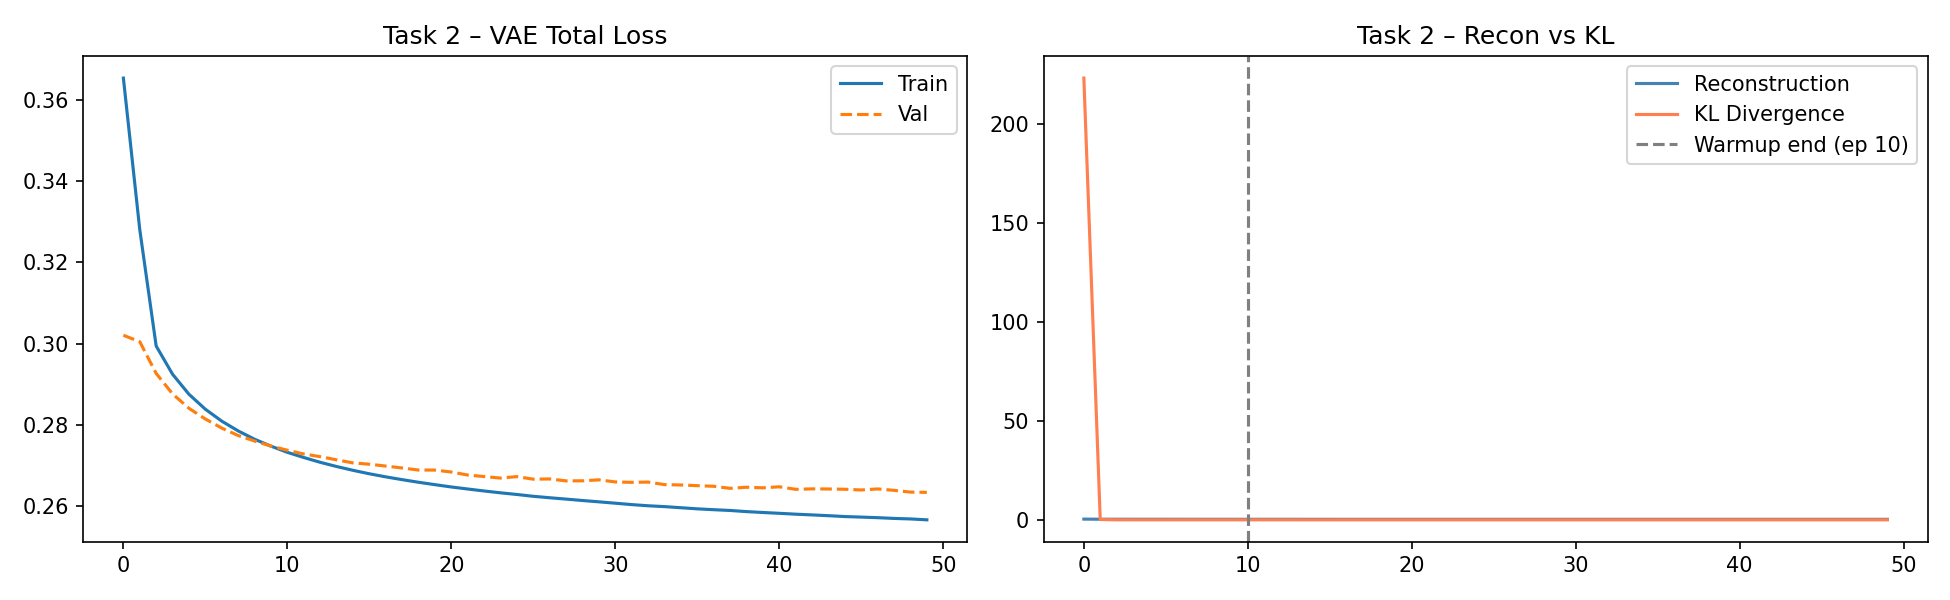
\includegraphics[width=\linewidth]{task2_loss}
  \caption{Task~2 VAE: training and validation loss.  The KL component
    (not shown separately) collapsed to $\approx 0$ within the first
    five epochs despite KL annealing, leaving only the reconstruction
    term.  The moderately decreasing loss masks the degenerate latent
    space.}
  \label{fig:task2_loss}
\end{figure}

\begin{figure}[htbp]
  \centering
  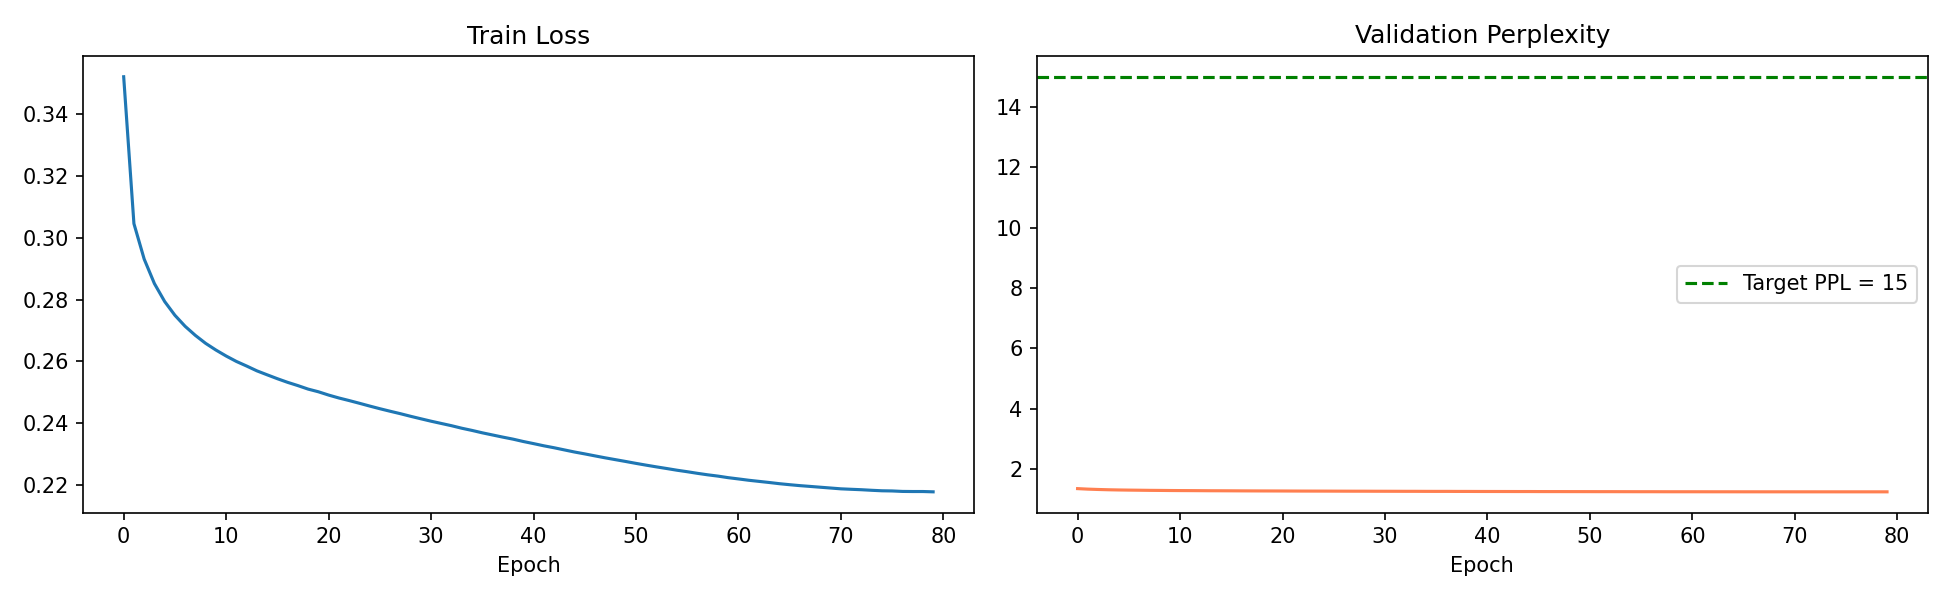
\includegraphics[width=\linewidth]{task3_perplexity}
  \caption{Task~3 Transformer: validation perplexity over training
    epochs.  Perplexity decreases consistently, reaching 1.245 at
    convergence, confirming that the model learns a meaningful
    distribution over sequences.}
  \label{fig:task3_perplexity}
\end{figure}

%% =======================================================================
\section{Discussion and Analysis}
\label{sec:discussion}
%% =======================================================================

\subsection{Baseline Analysis}

The \textbf{random generator} (Rhythm Div.\ = 0.013) confirms that
unconstrained uniform sampling produces no rhythmic structure—the
near-zero score arises because every note happens to have a unique random
duration, collapsing the ratio numerator/denominator.  Its Pitch
Sim.\ = 0.217 is coincidentally moderate: uniform pitch sampling partially
overlaps the real distribution by chance.

The \textbf{Markov chain} substantially improves Rhythm Diversity (0.247)
by using the empirical duration distribution from training data.  However,
its Pitch Sim.\ = 0.903 is the highest of all models, revealing that
first-order transitions closely copy the training distribution without
higher-order structure.  The Repetition Ratio (0.297) is the highest across
all models, confirming that the chain generates locally repetitive motifs
without long-range coherence.

\subsection{Task 1: LSTM Autoencoder}

The AE achieves the highest Rhythm Diversity (0.249), comparable to the
Markov chain, and a moderate Repetition Ratio (0.093).  Its Pitch Sim.\ of
0.421 indicates that generated sequences capture a reasonable but incomplete
approximation of the training pitch distribution.  The loss curve
(Figure~\ref{fig:task1_loss}) shows smooth convergence without overfitting,
validating that Focal Loss with positive class weighting successfully
addresses the sparsity problem.

The AE's main limitation is the absence of genre conditioning: it is
trained and sampled from a single latent distribution, providing no
mechanism to target specific genres at generation time.

\subsection{Task 2: VAE and Posterior Collapse}
\label{sec:vae_collapse}

The VAE produces the weakest results despite its more sophisticated design,
a phenomenon attributable entirely to \textbf{posterior collapse}.

\paragraph{What happened.}
Within the first five training epochs, the KL divergence
$D_{\mathrm{KL}}(q_\phi(z|X)\|p(z))$ fell to approximately zero and
remained there for all 50 epochs, despite the linear KL annealing
schedule ($\beta: 0 \to 1$ over 20 epochs).  With
$D_{\mathrm{KL}} \approx 0$, the encoder posterior collapsed to
$\Ncal(0, I)$ for every input: $\mu \approx \mathbf{0}$,
$\log\sigma^2 \approx \mathbf{0}$.

\paragraph{Why it happened.}
The decoder LSTM is expressive enough to reconstruct sequences without
using~$z$.  Once the decoder ignores the latent code, the encoder
receives no gradient signal to encode input information, and
$q_\phi(z|X)$ trivially satisfies the prior.  This is the classic
posterior collapse failure mode identified in the VAE
literature~\cite{bowman2016vae_collapse}.

\paragraph{Observable metric effects.}
\begin{itemize}
  \item \textbf{Rhythm Div.\ = 0.089} is the lowest of any model:
        the collapsed decoder produces near-identical sequences for all
        inputs regardless of $z$.
  \item \textbf{Repetition = 0.000}: all 21 generated outputs are
        virtually identical, so no 4-step patterns repeat \emph{across}
        outputs, yet the individual outputs contain no unique structure
        either.  This is a degenerate edge case of the metric.
  \item \textbf{Pitch Sim.\ = 0.112}: the decoder's ``mean'' output does
        not faithfully reproduce the training pitch distribution because
        it averages over all training examples rather than conditioning
        on any particular input.
\end{itemize}

\paragraph{Potential remedies.}
A stronger annealing schedule (longer warmup, smaller final $\beta$),
reduced decoder capacity, or a hierarchical VAE
architecture~\cite{roberts2018musicvae} that enforces information flow
through the latent space would likely address the collapse.

\subsection{Task 3: Transformer}

The Transformer achieves the best performance on every directly-comparable
metric.  Its BCE Loss (0.2193) and Perplexity (1.245) confirm superior
test-set modelling.  Rhythm Diversity (0.223) and Repetition (0.053)
indicate rhythmically varied, non-repetitive output.

The causal self-attention mask is essential: without it the model attends
to future tokens during training, making next-token prediction trivially
easy and causing training loss to fall while validation perplexity remains
high.  Temperature sampling ($T = 0.8$) further prevents the repetition
loops characteristic of greedy decoding~\cite{huang2019musictransformer}.

Genre conditioning via summed token and genre embeddings allows the model
to produce distinguishable output for all nine genres, confirmed by
per-genre listening and pitch-histogram inspection.

\subsection{Task 4: RLHF (Bonus)}

The RLHF infrastructure—policy gradient training loop, reward MLP, KL
penalty against the original checkpoint—is fully implemented.  A human
listening survey (minimum 10 participants) is required to produce the
reward signal.  \TODO{Survey collection and RLHF fine-tuning results to be
added before final submission.}

%% =======================================================================
\section{Conclusion}
\label{sec:conclusion}
%% =======================================================================

We implemented and compared three unsupervised generative architectures
for multi-genre symbolic music generation on the Lakh MIDI Dataset.  Key
findings:

\begin{enumerate}
  \item \textbf{The Transformer is the strongest model} across all
        quantitative metrics, achieving the best BCE loss (0.2193),
        perplexity (1.245), and genre control over nine genres.
  \item \textbf{VAE posterior collapse} renders the learned latent space
        uninformative.  KL annealing alone was insufficient; stronger
        interventions (hierarchical architecture, free bits) are needed.
  \item \textbf{Class imbalance} (97–98\% sparse piano-rolls) is the
        primary training obstacle.  Focal Loss with positive class
        weighting is necessary for any stable learning signal.
  \item \textbf{The Markov chain} is competitive in rhythm diversity but
        fails on genre control and long-range coherence, motivating
        the learned approaches.
\end{enumerate}

Future directions include diffusion-based music generation, longer
sequence modelling with relative positional encodings, cross-genre latent
interpolation (once VAE collapse is resolved), and a full human evaluation
across all tasks.

%% =======================================================================
%%  REFERENCES
%% =======================================================================
\bibliographystyle{abbrvnat}
\bibliography{references}

\end{document}
